% DO NOT COMPILE THIS FILE DIRECTLY!
% This is included by the other .tex files.

\begin{frame}[t,plain]
\titlepage
\end{frame}

\section{MISP in general}

\begin{frame}
    \frametitle{about CIRCL and MISP}
    \begin{itemize}
        \item CIRCL
        \begin{itemize}
            \item National CERT for the private sector, communes, non-govermental entities in Luxembourg
            \item Government-driven initiative, funded by the Ministry of Economy
            \item Mission is to provide a systematic response to computer security threats and incidents
            \item Open Source toolsmiths
        \end{itemize}
        \item Our relationship with MISP has two sides
        \begin{itemize}
            \item We {\bf lead the development} of the MISP platform
            \item We are also involved with and {\bf run several communities}
        \end{itemize}
    \end{itemize}
\end{frame}

\begin{frame}
\frametitle{Before we start - What is MISP?}
\begin{itemize}
       \item MISP is a {\bf threat information sharing} platform
       \item A tool that {\bf collects} information from partners, your analysts, your tools, feeds
       \item Normalises, {\bf correlates}, {\bf enriches} the data
       \item Allows teams and communities to {\bf collaborate}
       \item {\bf Feeds} automated protective tools and analyst tools with the output
\end{itemize}
\end{frame}

\begin{frame}
\frametitle{Before we start - what is MISP?}
\begin{itemize}
        \item It is also a set of {\bf open standards} implemented both by MISP and other tools
        \item Additionally, it is an {\bf ecosystem} of libraries, supporting tools
        \item A collection of guidance and best practice documentation by practitioners
        \item All of these are free \& open source
\end{itemize}
\end{frame}

\begin{frame}
\frametitle{What are the objectives of a modern TISP?}      
\begin{itemize}
       \item A tool that {\bf collects} information from partners, your analysts, your tools, sensors, feeds
       \item Normalises, {\bf correlates}, {\bf enriches} the data
       \item Manages your processes and automates tasks such as {\bf notifications}, {\bf data flow management}, {\bf triaging} and so on
       \item Allows teams and communities to {\bf collaborate} and rapidly {\bf exchange knowledge}
       \item {\bf Feeds} automated protective tools and analyst tools with the output
       \item {\bf Presents} both individualised and community centric facts, trends, reports of the intelligence
\end{itemize}
\end{frame}


\begin{frame}
 \frametitle{MISP: Started from a practical use-case}
 \begin{itemize}
         \item During a malware analysis workgroup in 2012, we discovered that we worked on the analysis of the same malware.
         \item We wanted to share information in an easy and automated way {\bf to avoid duplication of work}.
         \item Christophe Vandeplas (then working at the CERT for the Belgian MoD) showed us his work on a platform that later became MISP.
         \item A first version of the MISP Platform was used by the MALWG and {\bf the increasing feedback of users} helped us to build an improved platform.
         \item MISP is now {\bf a community-driven development} supporting different intelligence communities.
 \end{itemize}
\end{frame}

\begin{frame}
\frametitle{Development based on practical user feedback}
\begin{itemize}
\item There are many different types of users of an information sharing platform like MISP:
        \begin{itemize}
                \item {\bf Malware reversers} willing to share indicators of analysis with respective colleagues.
                \item {\bf Security analysts} searching, validating and using indicators in operational security.
                \item {\bf Intelligence analysts} gathering information about specific adversary groups.
                \item {\bf Law-enforcement} relying on indicators to support or bootstrap their DFIR cases.
                \item {\bf Risk analysis teams} willing to know about the new threats, likelyhood and occurences.
                \item {\bf Fraud analysts} willing to share financial indicators to detect financial frauds.
                \item {\bf Military} sharing highly specialised information.
        \end{itemize}
\end{itemize}
\end{frame}

        
\begin{frame}
\frametitle{Why do we develop all of this?}      
\begin{itemize}
   \item {\bf Main goal}: Make our own lives and the lives of our constituency easier
   \begin{itemize}
       \item Our central tool for ingesting, storing and disseminating information...
       \item ...as well as to interact with organisations
       \item By solving issues of other communities, we already have them prepared for information sharing with us when needed
   \end{itemize}
   \item {\bf Secondary}: Democratise threat intelligence for all
   \item {\bf Stretch goal}: Build a full open-source tool-chain for CSIRTs / SoCs / etc
\end{itemize}
\end{frame}

\begin{frame}
 \frametitle{Communities using MISP}
 \begin{itemize}
	 \item Communities are groups of users sharing within a set of common objectives/values.
	 \item CIRCL operates multiple MISP instances with a significant user base (more than 2k organizations with close to 5k users).
         \item {\bf Trust groups} running MISP communities in island mode (air gapped system) or partially connected mode.
	 \item {\bf Financial sector} (banks, ISACs, payment processing organizations) use MISP as a sharing mechanism.
	 \item {\bf Military and international organizations} (NATO, military CSIRTs, n/g CERTs,...).
	 \item {\bf Security vendors} running their own communities.
	 \item {\bf Sectorial communities} Telcoes, ISPs, Medical, ATF, ...
         \item {\bf Topical communities} set up to tackle individual specific issues (disinformation, SIGINT, COVID-19, ...)
 \end{itemize}
\end{frame}


\begin{frame}
\frametitle{Information pipeline}
    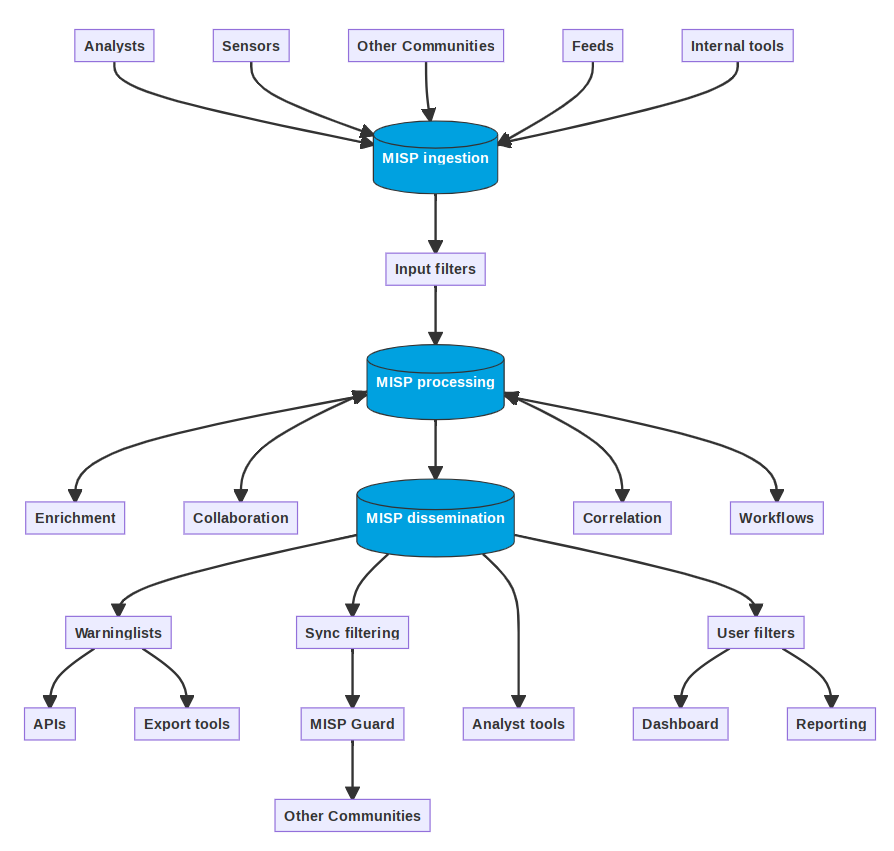
\includegraphics[width=0.75\linewidth]{misp_data_flow.png}
\end{frame}


\section{Some issues we try to tackle and their solutions}

\begin{frame}
\frametitle{Information quality management}
    \begin{itemize}
        \item What do we consider {\bf actionable intelligence}?
        \begin{itemize}
            \item Conflicting requirements - analyst work vs automated blocking for example
        \end{itemize}
        \item {\bf Filtering} both on {\bf input} and on {\bf output} separately
        \begin{itemize}
            \item Lax on ingestion, strict on output mantra
            \item Warninglists - sanitising obviously problematic data from output
            \item Indicator scoring / lifecycle management
        \end{itemize}
    \end{itemize}
\end{frame}

\begin{frame}
    \frametitle{Information quality management}
    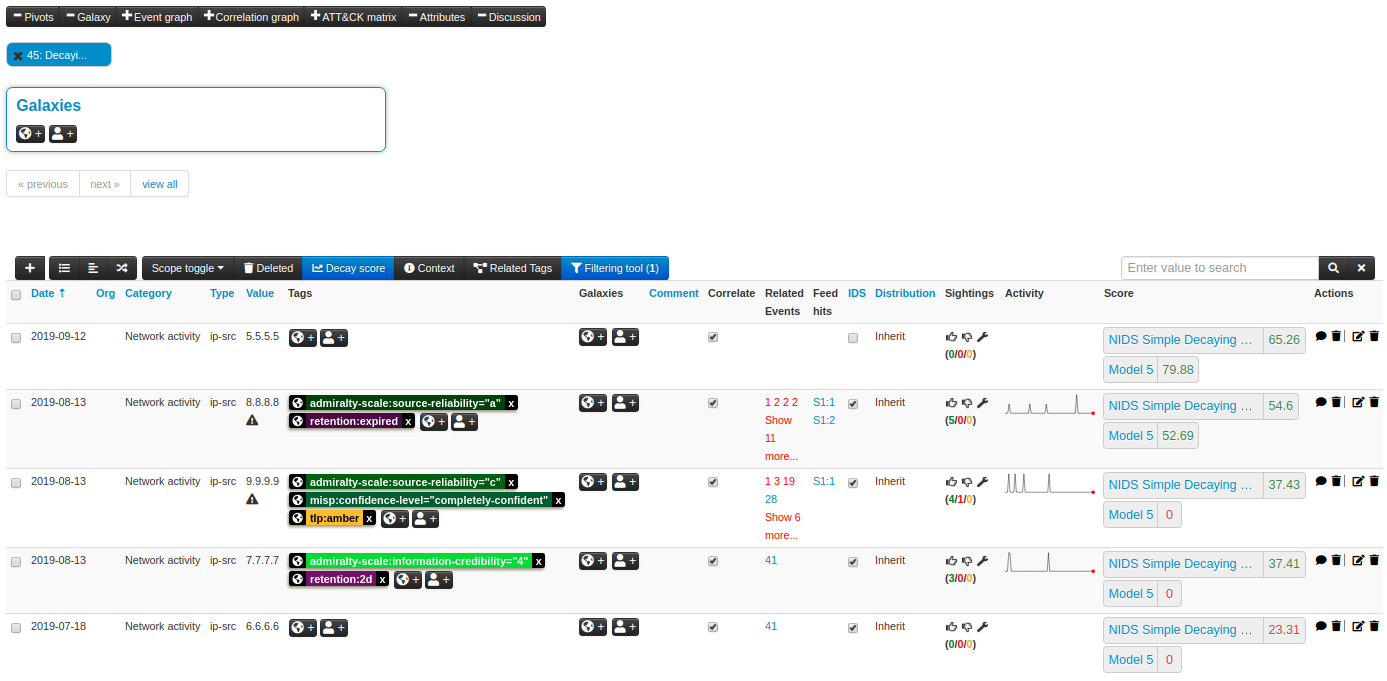
\includegraphics[width=1.00\linewidth]{decaying-event.png}
    \begin{itemize}
        \item {\bf Decay score} calculated based on the enabled models
        \item Score takes into account {\bf contextualisation, type, sightings}
    \end{itemize}
\end{frame}

\begin{frame}
    \frametitle{Information quality management}
    Customisable lifecycle management
    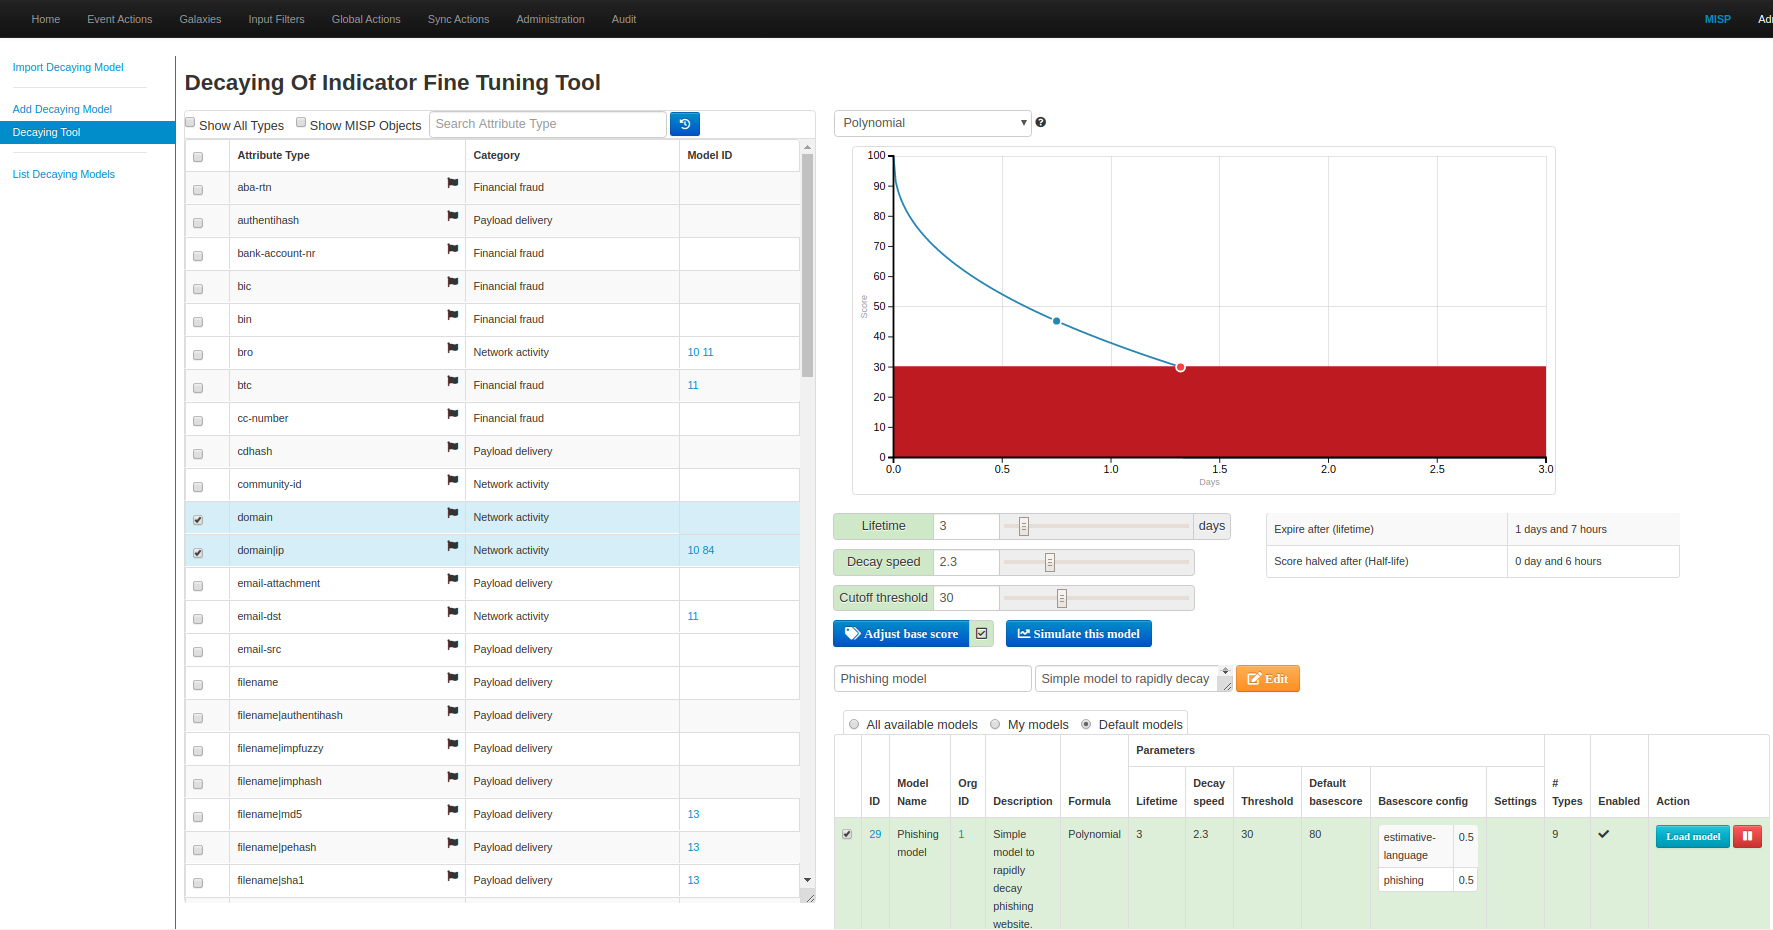
\includegraphics[width=1.00\linewidth]{decaying-tool.png}
\end{frame}



\begin{frame}
\frametitle{Drilling down into our data}
    \begin{itemize}
        \item Different use-cases require different tools.
        \item {\bf Interactive interaction} with the data
        \begin{itemize}
                \item "Event" tabular view
                \item "Event" graph view
                \item Correlation graphs
                \item Various search interfaces
        \end{itemize}
        \item {\bf Trends and overviews}
        \begin {itemize}
                \item Dashboarding
                \item ATT\&CK and similar frameworks based heatmaps
                \item Alert e-mails and periodic reporting
        \end{itemize}
    \end{itemize}
\end{frame}

\begin{frame}
    \frametitle{Drilling down into our data}
        \begin{center}
	    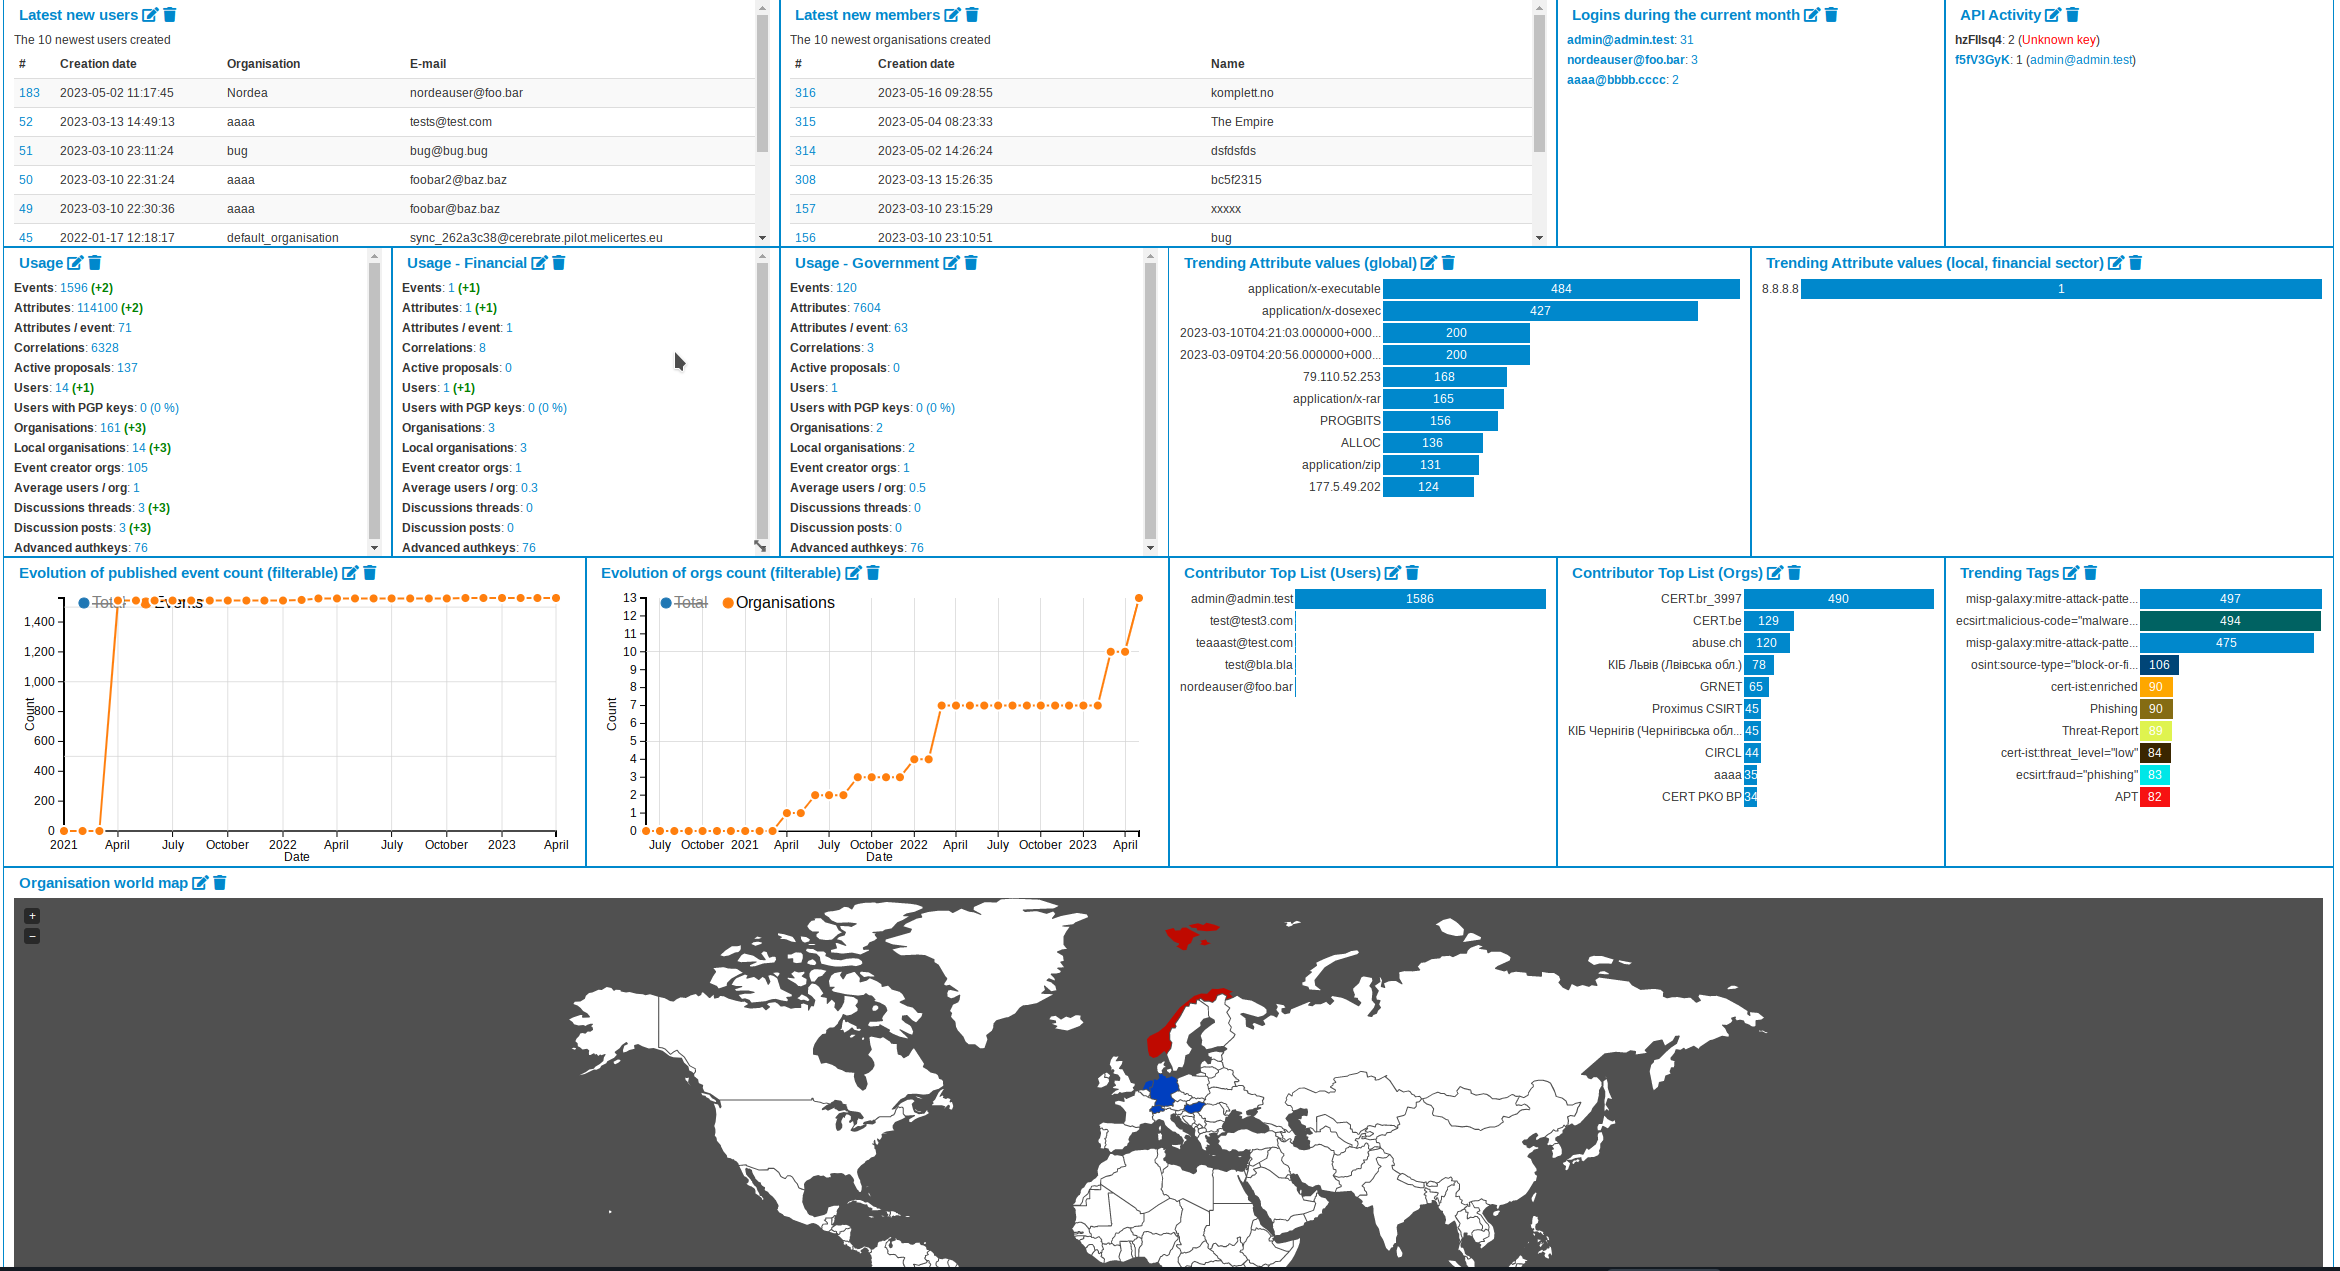
\includegraphics[width=1.05\linewidth]{dashboard-new.png}
        \end{center}
\end{frame}




\begin{frame}
\frametitle{Drilling down into our data}
    \begin{itemize}
        \item APIs
        \begin{itemize}
                \item Long list of {\bf filters}
                \item {\bf Complex queries}
                \item Infusing queries with other tools ({\bf warninglists, decaying})
                \item Interactive {\bf UI query builder and tester}
        \end{itemize}
    \end{itemize}
\end{frame}


\begin{frame}
\frametitle{Data model management}
    \begin{itemize}
        \item Three tier approach to information
        \item All three tiers are tightly integrated with one another
        \begin{itemize}
            \item {\bf Data} (Attributes, Objects, Relationships)
            \item {\bf Knowledge} ("Galaxies", Labels)
            \item {\bf Analyst reports} (Markdown reports)
        \end{itemize}
        \item Different communities have wildly different requirements - extension mechanisms
        \begin{itemize}
            \item {\bf Object templates}
            \item Custom {\bf Galaxies}
            \item {\bf Taxonomies}
        \end{itemize}
    \end{itemize}
\end{frame}

\begin{frame}
    \frametitle{Data model management}
    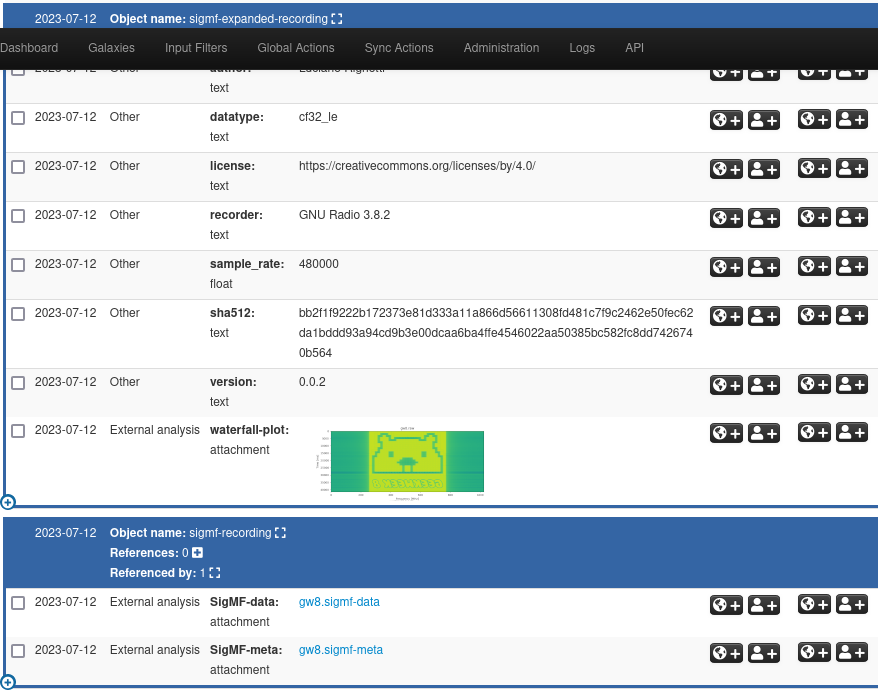
\includegraphics[width=0.90\linewidth]{sigint.png}
\end{frame}

\begin{frame}
\frametitle{Customising MISP}
    \begin{itemize}
        \item Highly configurable per community need
             \begin{itemize}
                 \item Hundreds of {\bf configuration options} to manage MISP behaviours
                 \item Hooking and modifying {\bf core funtionalities via Workflows}
                 \item Custom modules via companion system ({\bf MISP-modules})
                 \item {\bf Modular} parts of the {\bf codebase} (e-mail templates, dashboard elements, import/export functions)
                 \item If all of that is not enough - extensive {\bf Python library} support for DIY fans :)
             \end{itemize}
    \end{itemize}
\end{frame}

\begin{frame}
    \frametitle{Customising MISP}
    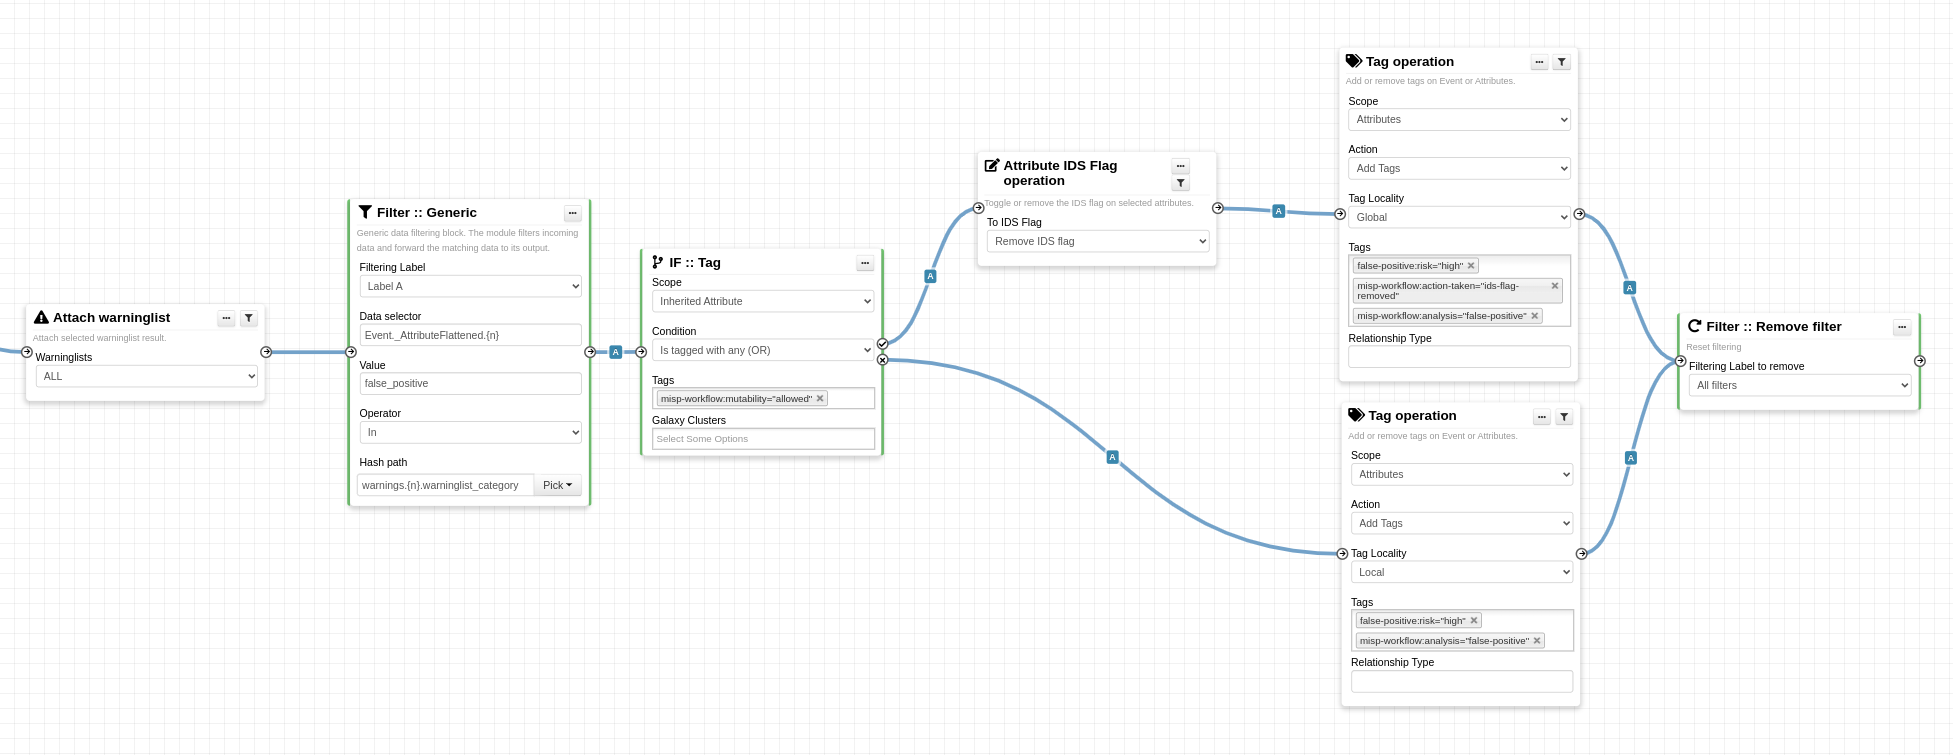
\includegraphics[width=1.00\linewidth]{blueprint.png}
\end{frame}


\section{Wrapping it all up}

\begin{frame}
\frametitle{Community driven effort}
    \begin{itemize}
        \item This concludes a {\bf brief glimpse into what MISP is} and some of the key issues to tackle
        \item MISP is evolving based on {\bf community efforts and needs}
        \item The outcome is a highly {\bf versatile and customisable} system
        \item We all have different ideas of what we'd like to be able to do in our TISP
        \item {\bf Prioritisation is hard} plus there are only so many hours in a day...
        \item ...{\bf Get involved}, let us know how we can make it better or at least usable for your use-case!
    \end{itemize}
\end{frame}


\begin{frame}
  \frametitle{Get in touch if you have any questions}
  \begin{itemize}
    \item Contact me:
    \begin{itemize}
      \item andras.iklody@circl.lu \url{https://twitter.com/iglocska} \url{https://infosec.exchange/@iglocska}
    \end{itemize}    
    \item Contact us:
    \begin{itemize}
      \item info@circl.lu \url{https://twitter.com/circl_lu} \url{https://www.circl.lu/}
      \item \url{https://github.com/MISP} \url{https://www.misp-project.org/}
      \item \url{https://twitter.com/MISPProject} \url{https://misp-community.org/@misp}
    \end{itemize}
  \end{itemize}
\end{frame}

